% This version of CVPR template is provided by Ming-Ming Cheng.
% Please leave an issue if you found a bug:
% https://github.com/MCG-NKU/CVPR_Template.

\documentclass[final]{cvpr}

\usepackage{times}
\usepackage{epsfig}
\usepackage{graphicx}
\usepackage{amsmath}
\usepackage{amssymb}
\usepackage[numbers]{natbib}
\usepackage{notoccite}
\usepackage{subcaption}
\captionsetup{compatibility=false}
\usepackage{graphicx}
\usepackage{fancyvrb}

\setlength{\abovecaptionskip}{-3pt plus 3pt minus 2pt}


% Include other packages here, before hyperref.

% If you comment hyperref and then uncomment it, you should delete
% egpaper.aux before re-running latex.  (Or just hit 'q' on the first latex
% run, let it finish, and you should be clear).
\usepackage[pagebackref=true,breaklinks=true,colorlinks,bookmarks=false]{hyperref}


\def\cvprPaperID{34} % *** Enter the CVPR Paper ID here
\def\confYear{CVPR 2021}
%\setcounter{page}{4321} % For final version only


\begin{document}
	
	%%%%%%%%% TITLE
	\title{Classification of Lymphocytosis from Blood Cells\\
		\vspace{1mm}
		\large \normalfont Deep Learning for Medical Imaging}
	
	\author{\textbf{Clément Grisi}\\
		École des Ponts ParisTech\\
		\small \url{grisi.clement@gmail.com}
	\and
	\textbf{Marius Schmidt-Mengin}\\
	École des Ponts ParisTech\\
	\small \url{marius.schmidt.mengin@gmail.com}
	}
	
	\maketitle
	
	\begin{abstract}
		In this report, we emphasize our work for the data challenge organized as part of the Deep Learning for Medical Imaging class. The goal of the challenge is to classify lymphocytosis from blood cells. Through iterations in model definition and data representation, we managed to get $0.96623$ classification accuracy on the academic leaderboard (rank 1).
	\end{abstract}
	
	\vspace{-3mm}
	
	\section{Introduction}
	
	Lymphocytosis is an increase in the number or proportion of lymphocytes in the blood. It's a common finding, which can be either a reaction to infection or acute stress (reactive), or the manifestation of a lymphoproliferative disorder -- a type of cancer of the lymphocytes (tumoral). In clinical practice, the diagnosis as either reactive or tumoral is performed by trained pathologists who visually inspect blood cells under a microscope. The final decision also takes into consideration clinical attributes such as age, gender, and lymphocyte count. In spite of being relatively fast and affordable, lymphocytosis diagnisis lacks reproducibility between experts. Additional clinical tests are often required to confirm the malignant nature of the lymphocytes. However, this analysis is relatively expensive and time-consuming, and therefore is not performed for every patient in practice. In this context, automatic classification has the potential to provide accurate and reproducible diagnosis, saving precious time and ressources by quickly identifying which patient should be referred for flow cytometry analysis.
	
	\section{Problem Definiton}
	
	\subsection{Dataset}
	
	Blood smears and patient attributes were collected from $204$ patients from the routine hematology laboratory of the Lyon SudUniversity Hospital. All included patients have a lymphocyte count above $4\times10^9/L$. The blood smears were automatically produced by a Sysmex automat tool, and the nucleated cells were automatically photographed with a DM-96 device. The training set consists of $142$ patients ($44$ reactive and $98$ malignant cases), and the testing set of $42$ patients. For each patient, we have access to dozens of images of lymphocytes, as well as the following clinical attributes: gender, age, and lymphocyte count.
	
	\subsection{Evalutation Metric} 
	
	This challenge is evaluated on balanced accuracy (BA), which normalizes true positive (TP) and true negative (TN) predictions by the number of positive and negative samples, respectively. In particular, if one denotes false positives as FP and false negatives as FN, we have:
	
	\vspace{-2mm}
	
	\begin{equation*}
		\begin{aligned}
			\text{Sensitivity} & = \dfrac{\text{TP}}{\text{TP}+\text{FN}} ,\quad 
			\text{Specificity} & = \dfrac{\text{TN}}{\text{TN}+\text{FP}}\\
		\end{aligned}
	\end{equation*}

	\begin{equation*}
		\begin{aligned}
			\text{BA} = \dfrac{\text{Sensitivity}+\text{Specificity}}{2}
		\end{aligned}
	\end{equation*}
		
	\vspace{2mm}
	
	\subsection{Weak Supervision through Multiple Instance Learning} 
	
	The idea of weakly supervised learning is to exploit coarse-grained annotations to automatically infer finer-grained information. Coarse-grained information is often readily available in the form of patient level labels, but finer grained annotations are more difficult to obtain. Without precise local annotations, classification models cannot be trained in a fully supervised manner. Therefore, various weakly supervised techniques have recently been developed to overcome this issue. One of these techniques relies on multiple instance learning (MIL), an existing framework largely used in classic computer vision that has recently showed state-of-the-art results in several medical imaging tasks \cite{hou_MIL}. \\
	\\
	Babenko \cite{mil} gives a good example to understand multiple instance learning. Imagine several people, each of them having a key chain that contains a few keys. Some of these people are able to enter a certain room, and some aren’t. The task is to predict whether or not a given key chain can open the door of that room. To solve this problem, one needs to find the exact key that is common to all the \textit{positive} key chains. If one can correctly identify this key, one can also correctly classify an entire key chain - \textit{positive} if it contains the required key, or \textit{negative} if it doesn't.\\
	\\
	Hence, the multiple instance learning framework allows the training of a classifier from weakly labeled data: instead of providing input-label pairs, labels $\ell_b$ are assigned to \emph{sets} or \emph{bags} of instances. In this setting, the true instance labels $\ell_i$ can be thought of as latent variables, as they are not known during training. In our case, we can assume that only a subset of the images available for a patient with tumoral lymphocytosis do carry the information necessary to correctly classify that patient. Identifying these special instances perfectly fits in the multiple instance learning framework.
	
	\section{Related Work}
	
	add 3-4 papers: Maria's, Paige's
	
	\section{Methodology}
	
	\subsection{Standard MIL Assumption} 
	
	Under the standard MIL assumption, \emph{positive} patients must contain at least one instance classified as \emph{positive}, while \emph{negative} patients, instead, must have all their instances classified as \emph{negative}.\\
	\\
	The full pipeline is described on Figure \ref{fig:mil_pipeline}. Each forward + backward pass can be broken down into two consecutive stages: 
	
	\begin{itemize}
		\setlength\itemsep{-.0em}
		\item the \emph{inference} phase: during \emph{inference}, the models' weights are frozen. Each instance is run through the network and assigned a number between $0$ and $1$: the more likely an instance to indicate tumoral lymphocytosis, the closer the number assigned to $1$. Once all the instances of a patient have been processed, they can be ranked according to their probability of being \emph{positive}. For each patient, the top-$1$ instance is selected for the second stage: the \emph{learning} phase.
		\item the \emph{learning} phase: we now allow the models' weights to be updated. Given the standard MIL assumption detailed above, one can expect the top-$1$ instance of a \emph{positive} patient to be \emph{positive}, and the top-$1$ instance of a \emph{negative} patient to be \emph{negative}. Hence, as we run the top-$1$ instance through the network, we assign them the label of the patient they come from and update the weights accordingly: the network adjusts its weights in order to assign high probabilities to the top-$1$ instances coming from positive patients, while keeping low probabilities for the top-$1$ instances in negative patients. 
	\end{itemize}
	\noindent
	 At this stage, you might be wondering ``\textit{how this model converges} ?". It is true that it is not obvious as the model is initialized with ImageNet pre-trained weights, hence there's not reason to believe the model will assign high probabilities to the true positive instances, and low probabilities to true negative instances. And actually, the model does start by assigning random probabilities to each instances!  \\
	 \\
	 To understand how the model gradually learns to discriminate positive instances from negative ones, we need to focus on negative patients, who play a key role in the early stages of training. Under the standard MIL assumption , we know these patients must have all their instances classified as negative. At the end of the first \textit{inference} phase, the model has assigned these instances random probabilities, which can be either high or low. Hence, the top-$1$ instance for negative patient is random. I claim that this doesn't matter. Let me explain you why. What's important is what happens during the first \textit{learning} phase: for each negative patient, we have a (random) instance, which is negative. The model must adjust its weights to assign lower probabilities to each negative instances, such that at the following \textit{inference} step, all instances that look similar to negative instances will be assigned lower probabilities. As a result, all negative instances start to be assigned low probabilities, and positive instances will srand out, with higher probabilities. At this point, the top-$1$ instance of positive patient is more likely to be a true positive. And the model will adjust its weights to assign higher probabilities to this type of instance.\\
	 \\
	 This simplified reasoning allows to understand	how the model gently learns to discriminate suspicious instances from non-suspicious ones, and automatically infers fine-grained information from coarse-grained labels.\\
	 \\
	 \textcolor{red}{quick sentence to explain why using solely to top-$1$ instance might be, in some cases, problematic. this motivates the introduction of a hyperparameter $k$ whcih controls how many positive instances there might be in a positive bag (different degrees of positivity: 4 moderate positive instances, top proba is 0.6)}

	\subsection{Extended  MIL Assumption} 
	
	top-$k$ = hyperparameter

	\subsection{Taking More Tiles into Consideration}
	
	top-$k$ \& bottom-$k$
	
	\subsection{Taking All Tiles into Consideration}

	
	\section{Architecture}
	
	We start from a simple baseline and we evaluate different modifications.
	For each configuration, we run 10 trainings. Each training has its own seed for initializing the model and splitting the dataset (50/50 split). The 10 seeds are kept the same for each configuration. Each model is trained for 40 epochs with a batch size of 16, resulting in 5 batches per epoch. Evaluation if performed at the end of every epoch. We always optimize with Adam and a learning rate of $10^{-4}$. When we report a metric for any configuration, we average the 10 best values of each training, and again average this over all 10 trainings (the average is thus taken over 100 values). We always report 95\% confidence intervals.
	
	\subsection{Baseline}
	
	\begin{figure}[t]
		\begin{center}
			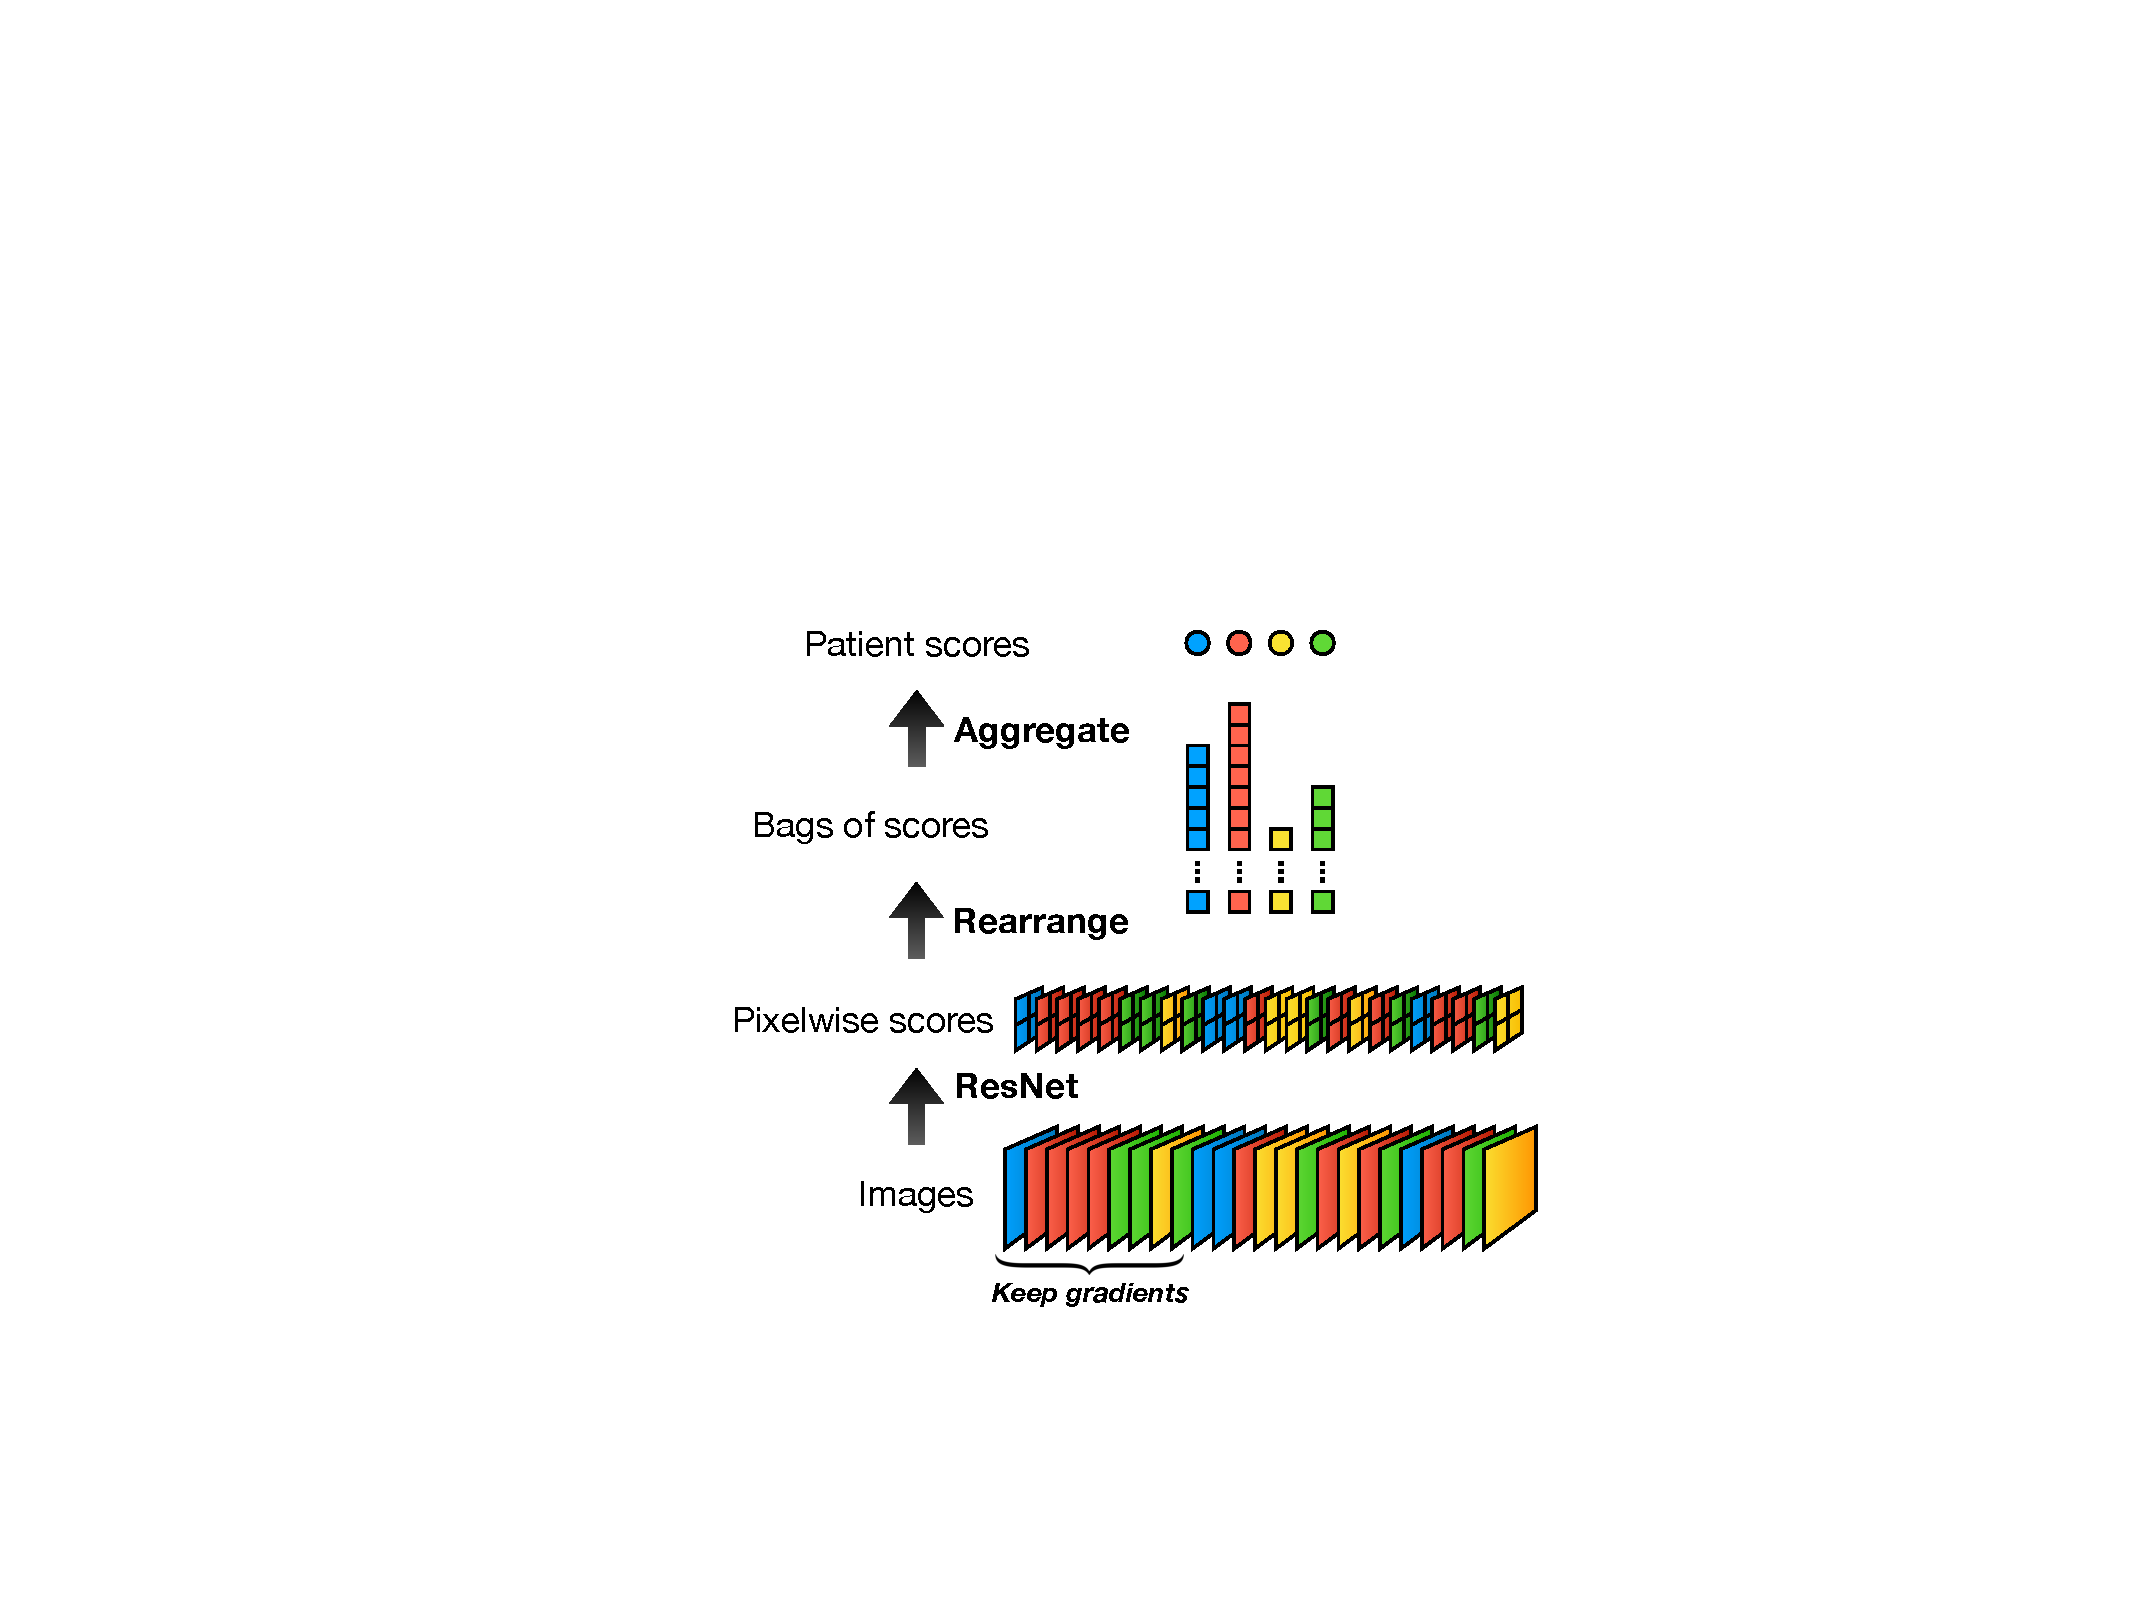
\includegraphics[width=0.9\linewidth]{fig/graphic2.pdf}
		\end{center}
		\caption{Baseline architecture.}
		\label{fig:overview}
	\end{figure}

	We adopt a simple and explainable architecture composed of a ResNet \cite{resnet} backbone followed by an aggregation module.
	For a given batch of patients, we take all their images and stack them into a batch.
	This batch is passed independently the backbone, without global pooling. 
	A $1\times 1$ convolution with one output channel is then applied to the resulting feature maps to obtain pixelwise prediction logits.
	These logits are rearranged into bags of scores, each bag corresponding to all  prediction for one patient.
	Finally, the aggregation module transforms each bag of scores into a final patient prediction.
	
	It is common that the features are aggregated before being linearly mapped to the final prediction score.
	In contrast, we apply the aggregation after reducing each feature to a single prediction logit. We did not find this to impact the results (and in the case where the aggregation function is linear, both methods are equivalent). Doing so makes the model more interpretable as each pixel (in the feature space) of each image can be given a score. 
	

	As the number of images passed through the backbone is often large, we keep the gradients for only a random subset of these images. Pseudo-code for this is provided by Algorithm 1.


\begin{table}[h]
	\renewcommand\tablename{Pseudo-code}
	\begin{Verbatim}[fontsize=\footnotesize, samepage=true, frame=single]
B, 3, H, W = image_batch.shape
max_forward_size = 512
max_backward_size = 512
features = []
i = 0
# forward images without keeping gradients
with torch.no_grad():
  while i < B - max_backward_size:
    j = min(i+max_forward_size,
            num_images-max_backward_size)
    features.append(backbone(images[i:j]))
    i = j
# forward image with gradients
features.append(backbone(images[i:]))
# Note: the images are supposed to be shuffled
# so that the subset for which the gradients
# are kept is random.
	\end{Verbatim}
    \caption{PyTorch-like pseudo-code for propagating the gradients through only a subset of the images, in order to not run out of GPU memory.}
	\label{alg1}
\end{table}




\subsection{Augmentations}
As the images are centered on a lymphocytes, we always apply a center crop of size 112 to all images (training, validation and testing). Initial experiments showed that this significantly improves the accuracy and reduces the computational resources. We use vertical and horizontal random flipping. We tried to use more agressive augmentations such as affine transforms and color jittering but this heavily impaired the accuracy.

\subsection{Backbone Choice}
We compared three backbones: ResNet18, ResNet34 and ResNet50 \cite{resnet}. We also tried a more recent backbone, EfficientNet \cite{efn}, but did not obtain good results.
The results are summarized in Figure \ref{fig:resnet}. ResNet18 achieves the best validation balanced accuracy. We use it for all our subsequent experiments.

\begin{figure}[t]
	\begin{center}
		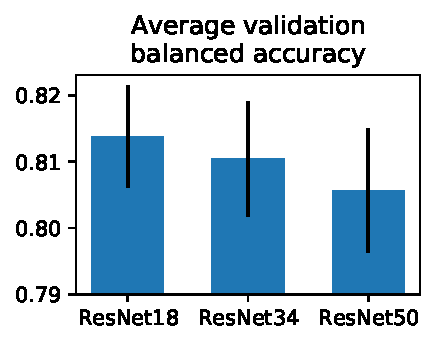
\includegraphics[width=0.47\linewidth]{fig/resnets_bal_acc.pdf}
		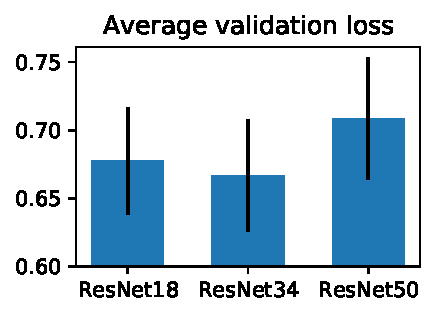
\includegraphics[width=0.47\linewidth]{fig/resnets_val_loss.pdf}
	\end{center}
	\caption{Impact of ResNet depth on validation loss and balanced accuracy. The black bars indicate 95\% confidence intervals. Shallower seems to be better but the results are not very significative.}
	\label{fig:resnet}
\end{figure}


	\subsection{Aggregation Function}

Let us denote all the predictions (logits) for patient $j$ by $\ell_i^j$, $\: i=1 \dots n_j$.
To aggregate these predictions, we seek to define some weights $\alpha_i^j \geq 0$ such that we can compute the final prediction logit for patient $j$ by
$$\ell^j = \sum_{i=1}^{n_j} \alpha_i^j \ell_i^j$$
(we assume that $\sum_i \alpha_i^j = 1$).
The confidence score is then given by applying the sigmoid function: $y_j = \sigma(l^j)$.
Two very common aggregation functions are the arithmetic mean and the maximum, where we would respectively set $\alpha_i^j = 1/n_j$ and $\alpha_i^j = \left\{ 1 \text{ if } \ell_i^j = \max_k \ell_k^j \text{ and } 0 \text{ otherwise}\right\}$.

We believe that these two aggregation function suffer from different problems. Let us express the gradient of the cross-entropy loss with respect to the logits $\ell_i^j$:
$$\frac{\partial L_{\text{CE}}}{\partial \ell_i^j} = \alpha_i^j \left(y^j - \bar{y}^j\right)$$
The maximum function results in sparse gradients (only one $\alpha_i^j$ is nonzero), as only the image that effectively generated the maximum produces a nonzero gradient. On the other hand, the mean function generates equal gradients for all images (all $\alpha_i^j$ are equal to $1/n_j$), meaning that for a positive patients, the "pull" generated by the gradient on negative images (if there are any) is equal to the pull applied to positive images. We developped an aggregation function that intuitively overcomes this problem.
The idea behind it is similar to focal loss \cite{focal}, which scales the weight so as to put more gradient on predictions that are deemed important in the context of a heavy class imbalance.
Our aggregation function defines the weights $\alpha_i^j$ by batch normalization \cite{bn} followed by the sigmoid function:
$$ \alpha_i^j = \sigma\left(\beta + \gamma \frac{\widetilde{\ell_i^j} - \mu}{\sqrt{V+\epsilon}}\right) $$
where $\; \widetilde{\text{ }} \;$ denotes the stop gradient operation (as in focal loss, no gradients are propagated through the weights), $\gamma$ and $\beta$ are trainable parameters, $\epsilon$ is a small constant and $\mu$ and $V$ are respectively the mean and variance of the logits $\ell_i^j$ over a batch of patients:
$$\mu = \tfrac 1 {n_1+\dots+n_B} \sum_{j=1}^{B} \sum_{i=1}^{n_j} \ell_i^j$$
$$V = \tfrac 1 {n_1+\dots+n_B} \sum_{j=1}^{B} \sum_{i=1}^{n_j} \left(\ell_i^j - \mu \right)^2$$
where $B$ is the batch size. Intuitively, $\alpha_i^j$ is small when $\ell_i^j$ is small compared to the rest of the batch, i.e, when it is likely to be a negative sample.

\begin{table}[h]
	\renewcommand\tablename{Pseudo-code}
\begin{Verbatim}[fontsize=\footnotesize, samepage=true, frame=single]
logits = conv(features) # 1 channel
weights = bn(logits.detach())
weighted_logits = weights * logits
y = sigmoid(weighted_logits.sum()/weights.sum())
\end{Verbatim}
\label{alg2}
\caption{PyTorch-like pseudo-code for our custom aggregation function}
\end{table}

\begin{figure}[t]
	\begin{center}
		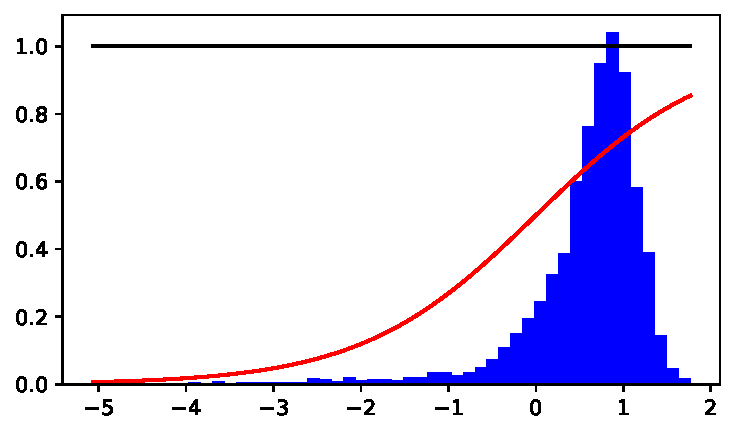
\includegraphics[width=0.95\linewidth]{fig/aggreg_2.pdf}
	\end{center}
	\caption{The distribution of the batch normalized logits over a bag is shown in blue. The red sigmoid shows the weight that is associated to each logit. The smaller the logit, the smaller the weight.}
	\label{fig:aggreg}
\end{figure}

\begin{figure}[t]
	\begin{center}
		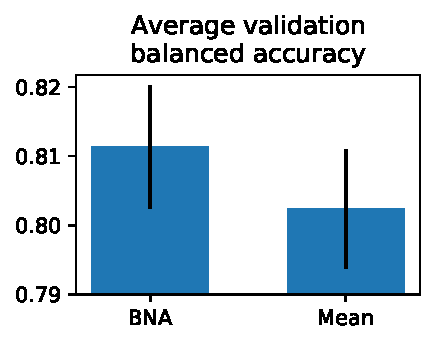
\includegraphics[width=0.47\linewidth]{fig/agg_bal_acc.pdf}
		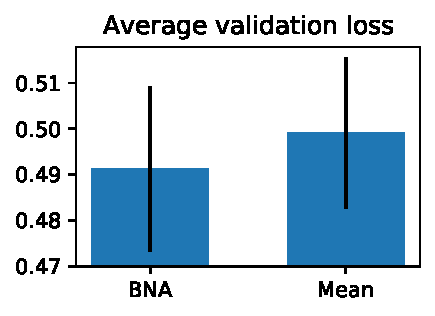
\includegraphics[width=0.47\linewidth]{fig/agg_val_loss.pdf}
	\end{center}
	\caption{Impact of our BN aggregation function on validation loss and balanced accuracy.  The black bars indicate 95\% confidence intervals.}
	\label{fig:resnet}
\end{figure}



\subsection{Number of images}
In the previous sections, when doing one training step, we used all the images of each patient and aggregated their logits.
In this experiment, we use only a small random subset of image per patient during each training step. 
We posit that selecting only a small subset of images provides some regularization to the training process. Indeed, assume that for a given positive patient, one image is easily identified by the network as positive. In this case, the network can ignore the other images. By selecting only a small random subset of images, we avoid this as the easy, positive images has a high probability of not being selected. Note that we implicitely make the assumption that in the case of a positive patient, a large number of images contains positive information.

	\section{Results}
	
	\section{Explainability}
	\begin{figure}[t]
		\begin{center}
			\includegraphics[width=0.7\linewidth]{fig/explainable1}
		\end{center}
		\caption{Predictions and images for 16 patients from the validation set. The patients where not cherry-picked. For each patient, a red left border indicates a positive ground truth label while green indicates a negative one. For each lymphocyte image, we provide on the left the $4\times 4$ predictions of the network. White means a score of one and black a score of 0.}
		\label{fig:resnet}
	\end{figure}
	
	\section{Conclusion}
	Future work: dilated ResNet ?\\
	Future work: aggregate embeddings using a recurrent neural network / self-attention encoder?
	
	\clearpage
	{\small
		\bibliographystyle{unsrt}
		\bibliography{egbib}
	}

\end{document}